
\label{sec:evaluation-metadata}

Nous avons ensuite procédé à l'évaluation de l'évolution de la consommation mémoire du document au cours des simulations, en fonction du \ac{CRDT} utilisé et du nombre de \emph{renaming bots}.
Nous présentons les résultats obtenus dans la \autoref{fig:evolution-document-size}.

\begin{figure}[!ht]
  \centering
  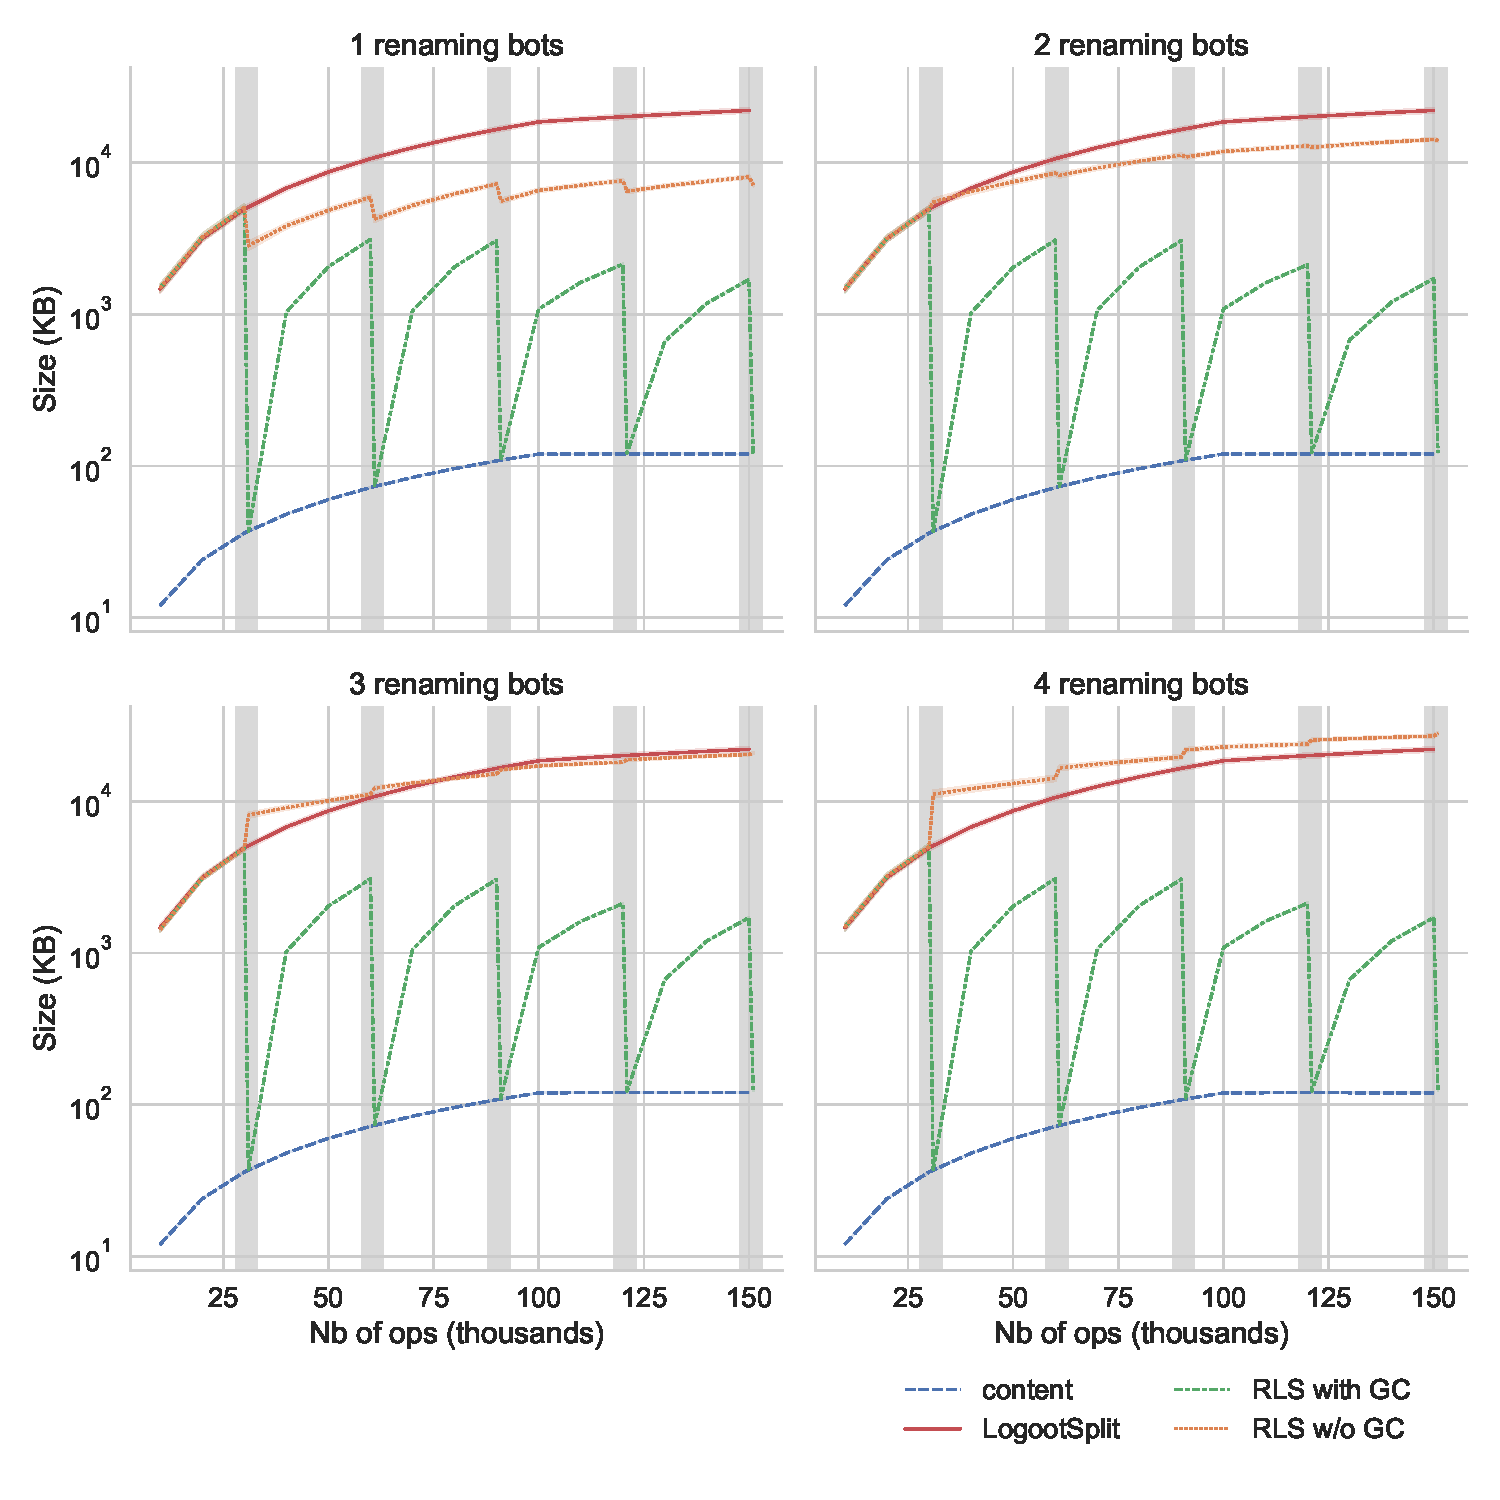
\includegraphics[width=\columnwidth]{img/2022-10-27-snapshot-sizes.pdf}
  \caption{Évolution de la taille du document en fonction du \ac{CRDT} utilisé et du nombre de \emph{renaming bots} dans la collaboration}
  \label{fig:evolution-document-size}
\end{figure}

Pour chaque graphique dans la \autoref{fig:evolution-document-size}, nous représentons 4 données différentes.
La ligne tiretée bleue correspond à la taille du contenu du document, \ie du texte, tandis que la ligne continue rouge représente la taille complète du document LogootSplit.

La ligne verte pointillée-tiretée représente la taille du document RenamableLogootSplit dans son meilleur cas.
Dans ce scénario, les noeuds considèrent que les opérations \emph{rename} sont causalement stables dès qu'ils les reçoivent.
Les noeuds peuvent alors bénéficier des effets du mécanisme de renommage tout en supprimant les métadonnées qu'il introduit : les \emph{anciens états} et époques.
Ce faisant, les noeuds peuvent minimiser de manière périodique le surcoût en métadonnées de la structure de données, indépendamment du nombre de \emph{renaming bots} et d'opérations \emph{rename} concurrentes générées.

La ligne pointillée orange représente la taille du document RenamableLogootSplit dans son pire cas.
Dans ce scénario, les noeuds considèrent que les opérations \emph{rename} ne deviennent jamais causalement stables.
Les noeuds doivent alors conserver de façon permanente les métadonnées introduites par le mécanisme de renommage.
Les performances de RenamableLogootSplit diminuent donc au fur et à mesure que le nombre de \emph{renaming bots} et d'opérations \emph{rename} générées augmente.
Néanmoins, même dans ces conditions, nous observons que RenamableLogootSplit offre de meilleures performances que LogootSplit tant que le nombre de \emph{renaming bots} reste faible (1 ou 2).
Ce résultat s'explique par le fait que le mécanisme de renommage permet aux noeuds de supprimer les métadonnées de la structure de données utilisée en interne pour représenter la séquence (\ie l'arbre AVL).

Pour récapituler les résultats présentés, le mécanisme de renommage introduit un surcoût temporaire en métadonnées qui augmente avec chaque opération \emph{rename}.
Mais ce surcoût se résorbe à terme une fois que le système devient quiescent et que les opérations \emph{rename} deviennent causalement stables.
Dans la \autoref{sec:offloading-former-states}, nous détaillerons l'idée que les \emph{anciens états} peuvent être déchargés sur le disque en attendant que la stabilité causale soit atteinte pour atténuer l'impact du surcoût temporaire en métadonnées.


